\documentclass[11pt, aspectratio=169]{beamer}

\usepackage{amsmath}
\usepackage[lined]{algorithm2e}
\usepackage{booktabs}
\usepackage{color}
\usepackage{csquotes}
\usepackage{fontspec}

%%%%%%%%%%%%%%%%%%%%%%%%%%%%%%%%%%%%%%%%%%%%%%%%%%%%%%%%
% Theme
%%%%%%%%%%%%%%%%%%%%%%%%%%%%%%%%%%%%%%%%%%%%%%%%%%%%%%%%

\usetheme[progressbar=frametitle]{metropolis}
\metroset{block=fill}
\metroset{sectionpage=progressbar}
\usefonttheme{professionalfonts}
\usepackage{theme/beamercolorthememetropolisinria}

%%%%%%%%%%%%%%%%%%%%%%%%%%%%%%%%%%%%%%%%%%%%%%%%%%%%%%%%
% Syntax highlighting
%%%%%%%%%%%%%%%%%%%%%%%%%%%%%%%%%%%%%%%%%%%%%%%%%%%%%%%%

\usepackage{minted}
\definecolor{codebg}{rgb}{0.95, 0.955, 0.96}

\setminted[bash]{
    autogobble,
    baselinestretch=1.2,
    bgcolor=codebg,
    fontsize=\footnotesize,
    framesep=50mm,
    xleftmargin=1em,
    xrightmargin=1em,
}

\setminted[python]{
    autogobble,
    baselinestretch=1.2,
    bgcolor=codebg,
    fontsize=\footnotesize,
    framesep=50mm,
    xleftmargin=0.5em,
    xrightmargin=0.5em,
}

%%%%%%%%%%%%%%%%%%%%%%%%%%%%%%%%%%%%%%%%%%%%%%%%%%%%%%%%
% Bibliography
%%%%%%%%%%%%%%%%%%%%%%%%%%%%%%%%%%%%%%%%%%%%%%%%%%%%%%%%

\usepackage[
    style=alphabetic,
    maxbibnames=99,
    maxcitenames=99,
]{biblatex}
\addbibresource{refs.bib}

%%%%%%%%%%%%%%%%%%%%%%%%%%%%%%%%%%%%%%%%%%%%%%%%%%%%%%%%
% Footnotes
%%%%%%%%%%%%%%%%%%%%%%%%%%%%%%%%%%%%%%%%%%%%%%%%%%%%%%%%

\newcommand\blfootcite[1]{%
    \invisible<1>{%
        {\color{white} \footfullcite{#1}}%
    }%
}

\newcommand\blfootcitetext[1]{%
    \invisible<1>{%
        \addtocounter{footnote}{-1}% assumes a footnotemark
        {\color{white} \footfullcite{#1}}%
    }%
}

\newcommand\blfootnote[1]{%
  \begingroup
  \renewcommand\thefootnote{}%
  \footnote{#1}%
  \addtocounter{footnote}{-1}%
  \endgroup
}

\newcommand\blfootnotetext[1]{%
  \begingroup
  \footnotetext{#1}%
  \endgroup
}

%%%%%%%%%%%%%%%%%%%%%%%%%%%%%%%%%%%%%%%%%%%%%%%%%%%%%%%%
% Abbreviations
%%%%%%%%%%%%%%%%%%%%%%%%%%%%%%%%%%%%%%%%%%%%%%%%%%%%%%%%

\def\eg{{\emph{e.g.}}}
\def\etal{{\emph{et al.}}}
\def\ie{{\emph{i.e.}}}
\def\xid{\dot{\xi}}

%%%%%%%%%%%%%%%%%%%%%%%%%%%%%%%%%%%%%%%%%%%%%%%%%%%%%%%%
% Metadata
%%%%%%%%%%%%%%%%%%%%%%%%%%%%%%%%%%%%%%%%%%%%%%%%%%%%%%%%

\title{
    Reinforcement learning for legged robots
}

\author{\textbf{St\'ephane Caron}}
\date{October 13, 2023}
\institute{Inria--\'{E}cole normale sup\'{e}rieure}

\begin{document}

\maketitle

%%%%%%%%%%%%%%%%%%%%%%%%%%%%%%%%%%%%%%%%%%%%%%%%%%%%%%%%%%%%%%%%%%%%%%%%%%%%%%%%

\section*{Robots with policies trained by RL}

\begin{frame}{2020: Quadrupedal locomotion~\cite{lee2020}}
    \vspace{1.5em}
    \begin{figure}
        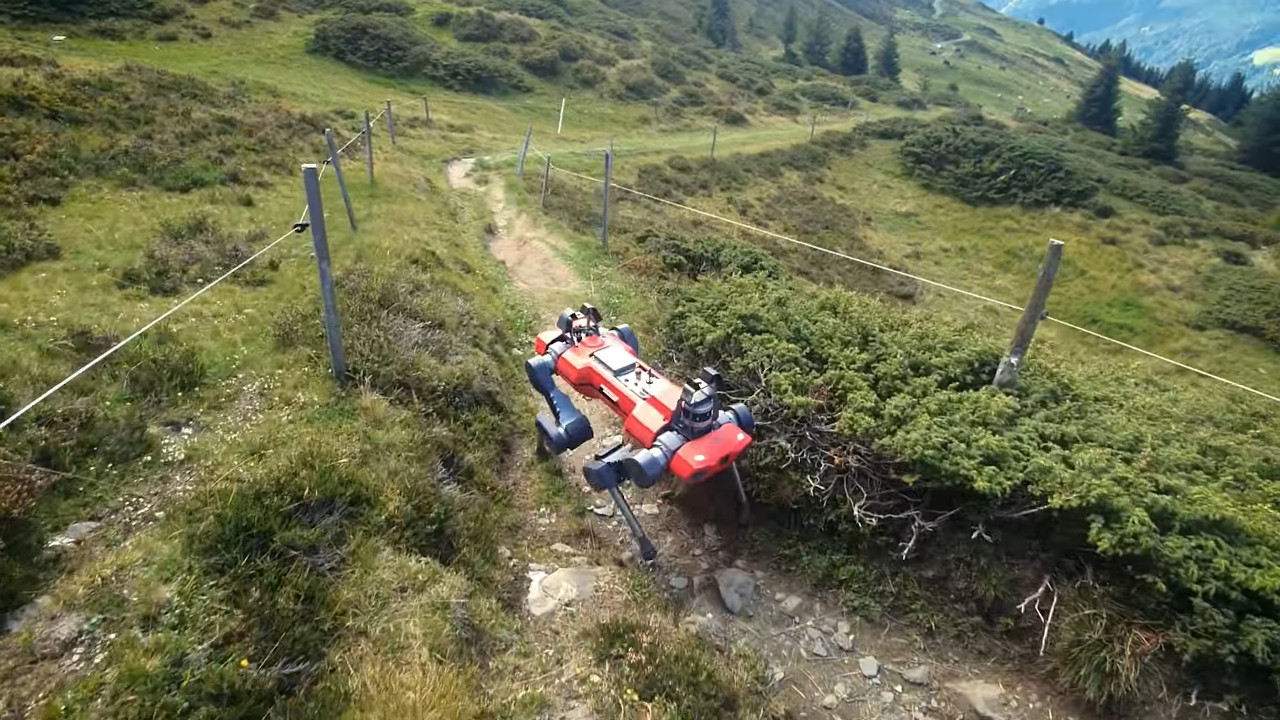
\includegraphics[height=5.5cm]{figures/hike-with-anymal.jpg}
    \end{figure}
    \begin{center}
        Teacher-student, residual reinforcement learning
    \end{center}
    \blfootnote{
        Video: \url{https://youtu.be/oPNkeoGMvAE}
    }
\end{frame}

\begin{frame}{2018: In-hand reorientation}
    \vspace{1.5em}
    \begin{figure}
        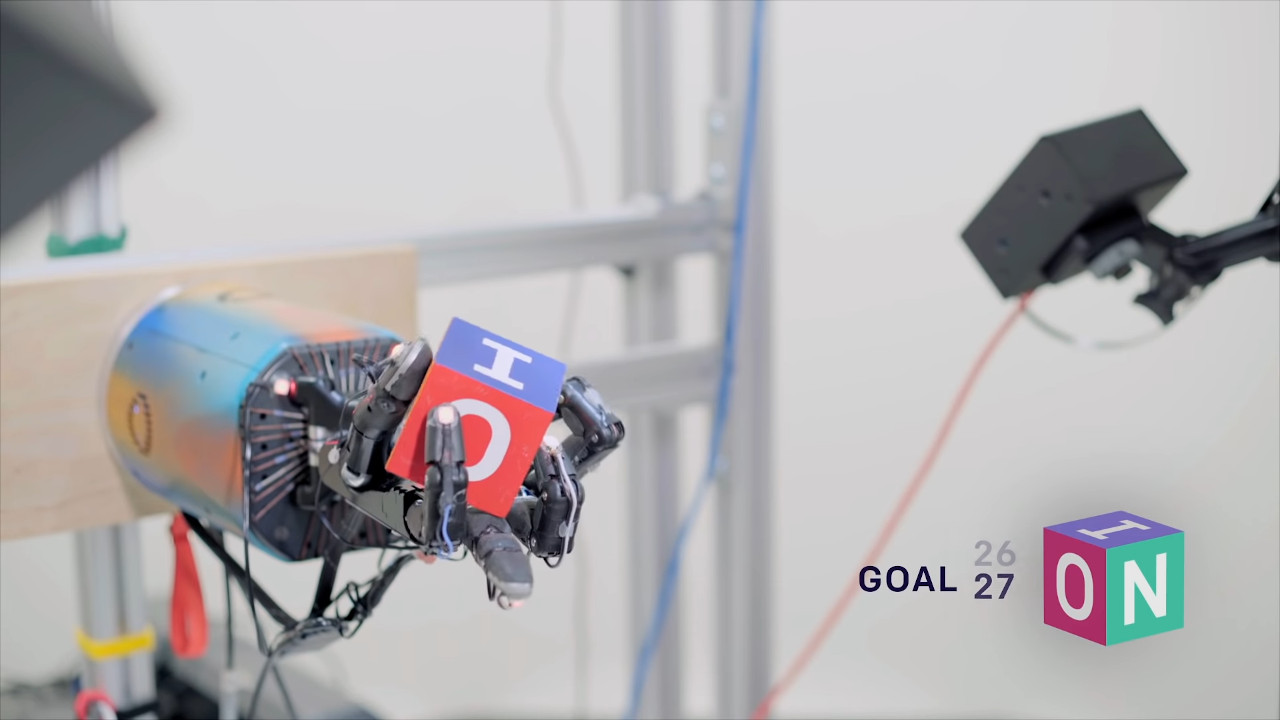
\includegraphics[height=5.5cm]{figures/in-hand-reorientation.jpg}
    \end{figure}
    \begin{center}
        Domain randomization, LSTM policy
    \end{center}
    \blfootnote{
        Video: \url{https://youtu.be/jwSbzNHGflM}
    }
\end{frame}

\begin{frame}{2010: Helicopter stunts}
    \vspace{1.5em}
    \begin{figure}
        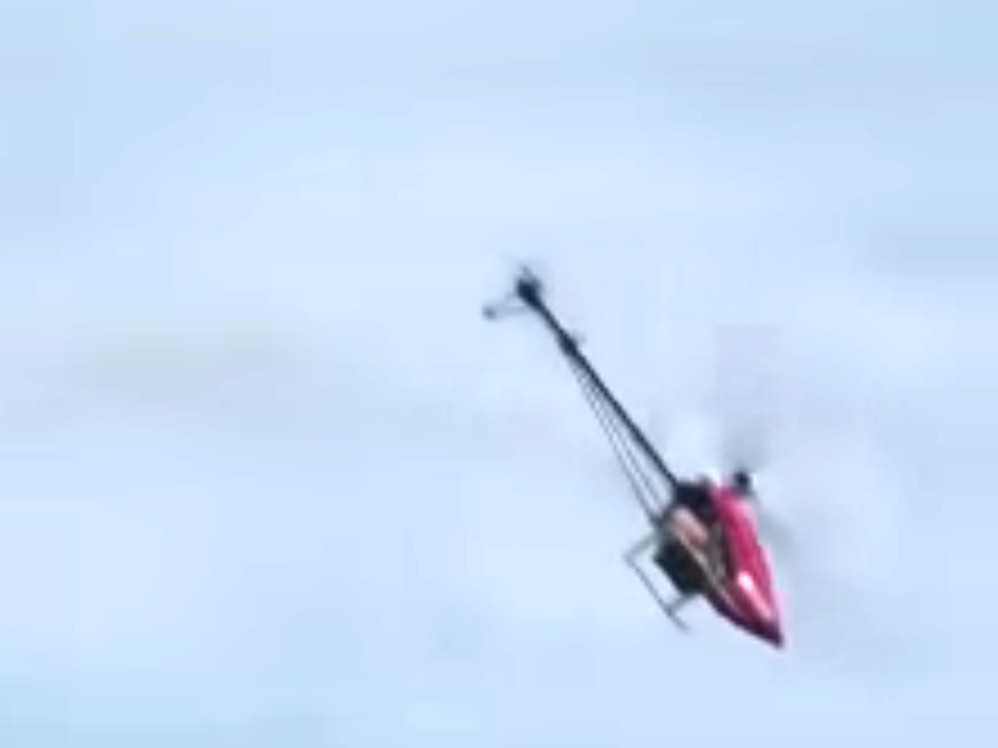
\includegraphics[height=3.5cm]{figures/helicopter-stunts.jpg}
    \end{figure}
    \begin{center}
        Autonomous Helicopter Aerobatics through Apprenticeship Learning~\cite{abbeel2010}
    \end{center}
    \blfootnote{
        Video: \url{https://youtu.be/M-QUkgk3HyE}
    }
\end{frame}

\begin{frame}{1997: Pendulum swing up~\cite{atkeson1997}}
    \vspace{1.5em}
    \begin{figure}
        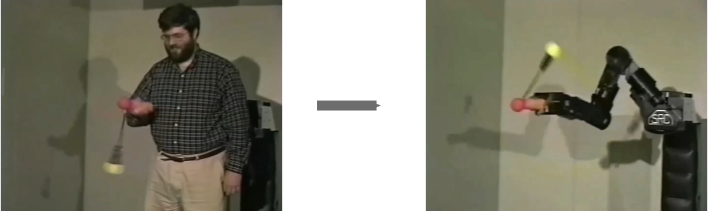
\includegraphics[height=3.5cm]{genfig/atkeson-demo.pdf}
    \end{figure}
    \blfootnote{
        Video: \url{https://youtu.be/g3I2VjeSQUM?t=294}
    }
\end{frame}

%%%%%%%%%%%%%%%%%%%%%%%%%%%%%%%%%%%%%%%%%%%%%%%%%%%%%%%%%%%%%%%%%%%%%%%%%%%%%%%%

\section*{Basics of reinforcement learning}

\begin{frame}{Scope}
    \begin{figure}
        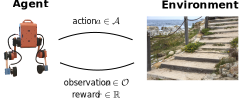
\includegraphics[height=5cm]{genfig/agent-environment.pdf}
    \end{figure}
\end{frame}

\begin{frame}{Rewards}
    \begin{figure}
        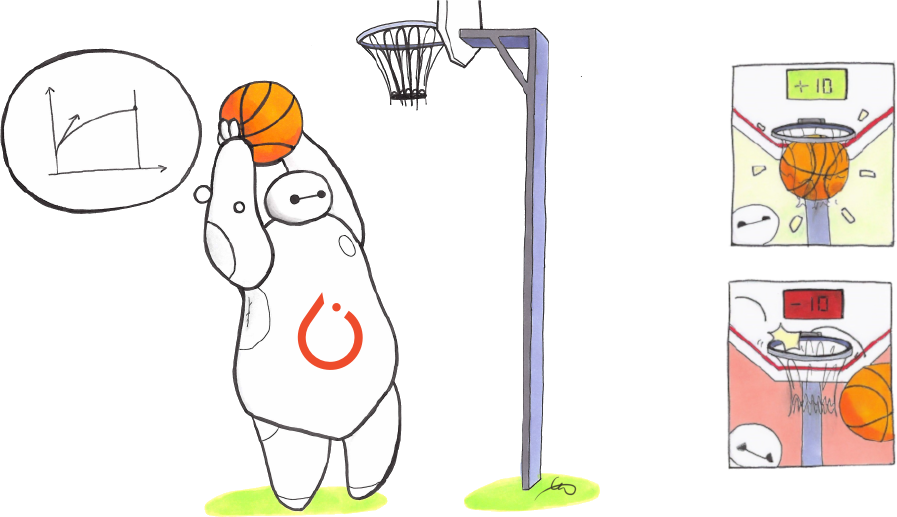
\includegraphics[height=5.5cm]{figures/stable-baselines3-logo.png}
    \end{figure}
    \blfootnote{
        Image credit: L. M. Tenkes, source: \url{https://araffin.github.io/post/sb3/}
    }
\end{frame}

\begin{frame}{Model of the environment}
    \begin{itemize}
        \item \textbf{State:} $s_t$, ground truth of the environment
        \item \textbf{Action:} $a_t$, decision of the agent
        \item \textbf{Observation:} $o_t$, \emph{partial} estimation of the state from sensors
        \item \textbf{Reward:} $r_t \in \mathbb{R}$, scalar feedback, often $r_t = r(s_t, a_t)$ or $r(s_t, a_t, s_{t+1})$
    \end{itemize}
    \vspace{-1em}
    \begin{table}
        \begin{tabular}{rlll}
            & \emph{Deterministic} & \emph{Stochastic} \\
            \hline
            \textbf{Model:} & $s_{t+1} = f(s_t, a_t)$ & $s_{t+1} \sim p(\cdot | s_t, a_t)$ & how the environment evolves \\
            \textbf{Initial state:} & $s_0$ & $s_0 \sim \rho_0(\cdot)$ & where we start from \\
            \textbf{Observation:} & $o_t = h(s_t)$ & $o_t \sim z(\cdot | s_t)$ & how sensors measure the world
        \end{tabular}
    \end{table}
    Altogether: partially-observable Markov decision process (POMPD).
\end{frame}

\begin{frame}{Model of the agent}
    A couple more definitions:
    \begin{itemize}
        \item \textbf{Episode:} $\tau = (s_0, a_0, s_1, a_1, \ldots)$
        \item \textbf{Return:} $R(\tau) = \sum_{t \in \tau} r_t$ or with discount $\gamma \in ]0, 1[$: $R(\tau) = \sum_{t \in \tau} \gamma^t r_t$
    \end{itemize}
    Finally, our model of the agent:
    \begin{itemize}
        \item \textbf{Policy:} agent decisions, deterministic $a_t = \pi(s_t)$ or stochastic $a_t \sim \pi(\cdot | s_t)$
    \end{itemize}
\end{frame}

\begin{frame}[fragile]{Example: The Gymnasium API}
    \begin{minted}{python}
        import gymnasium as gym
        import numpy as np

        with gym.make("UpkieGroundVelocity-v1", frequency=200.0) as env:
            env.reset() 
            action = np.zeros(env.action_space.shape)
            for step in range(1_000_000):
                observation, reward, terminated, truncated, _ = env.step(action)
                if terminated or truncated:
                    observation, _ = env.reset()
                pitch = observation[0]
                action[0] = 10.0 * pitch  # 1D action: [ground_velocity]
    \end{minted}
\end{frame}

\begin{frame}{Goal}
    The goal of reinforcement learning is to find a \emph{policy} that \emph{maximizes} return:
    \begin{align*}
        \max_{\pi} \ & \mathbb{E}_{\tau} [R(\tau)] \\
        \mathrm{s.t.} \ & \tau = (s_0, a_0, s_1, a_1, \ldots) \\
        & s_0 \sim \rho_0(\cdot) \\
        & a_0 \sim \pi(\cdot | s_0) \\
        & s_1 \sim f(\cdot | s_0, a_0) \\
        & \vdots
    \end{align*}
    \textbf{Shorthand:} $\max_\pi \mathbb{E}_{\tau \sim \pi}[R(\tau)]$.
\end{frame}

\begin{frame}{Parallel with control theory}
    \begin{table}
        \begin{tabular}{ll}
            \textbf{Reinforcement learning} & \textbf{Control theory} \\
            \hline
            State: $s_t$ & State: $x_t$ \\
            Observation: $o_t$ & Observation: $y_t$ \\
            Action: $a_t$ & Input: $u_t$ \\
            Reward: $r_t$ & Stage cost: $\ell(x_t, u_t)$ \\
            Episode: $\tau = (s_0, a_0, \ldots)$ & Trajectory: $\tau = (x_0, u_0, \ldots)$ \\
            Return: $\max R(\tau) = \sum_{t \in \tau} r_t$ & Cost: $\min J(\tau) = \sum_{t \in \tau} \ell(x_t, u_t)$ \\
            Model: $s_{t+1} = f(s_t, a_t)$ & Dynamics: $x_{t+1} = f(x_t, u_t)$ \\
        \end{tabular}
    \end{table}
\end{frame}

\begin{frame}{Value functions}
    State value functions:
    \begin{itemize}
        \item \textbf{On-policy value function:} return we can expect from a given policy: $V^\pi(s) = \mathbb{E}_{\tau \sim \pi}(R(\tau) | s_0 = s)$
        \item \textbf{Optimal value function:} best return we can expect from a state: $V^*(s) = \max_\pi \mathbb{E}_{\tau \sim \pi}(R(\tau) | s_0 = s)$
    \end{itemize}
    There are also state-action value functions $Q^\pi(s, a)$ and $Q^*(s, a)$.
\end{frame}

\begin{frame}{Components of an RL algorithm}
    A reinforcement-learning algorithm may include any of the following:
    \begin{itemize}
        \item \textbf{Policy:} behavior function
        \item \textbf{Value function:} evaluation of states
        \item \textbf{Model:} representation of the environment
    \end{itemize}
    An algorithm with a policy (actor) and a value function (critic) is called \emph{actor-critic}. If it doesn't use a model, it is \emph{model-free}. If it has one (e.g. chess, go), it is \emph{model-based}.
\end{frame}

\begin{frame}{A taxonomy of RL algorithms}
    \begin{figure}
        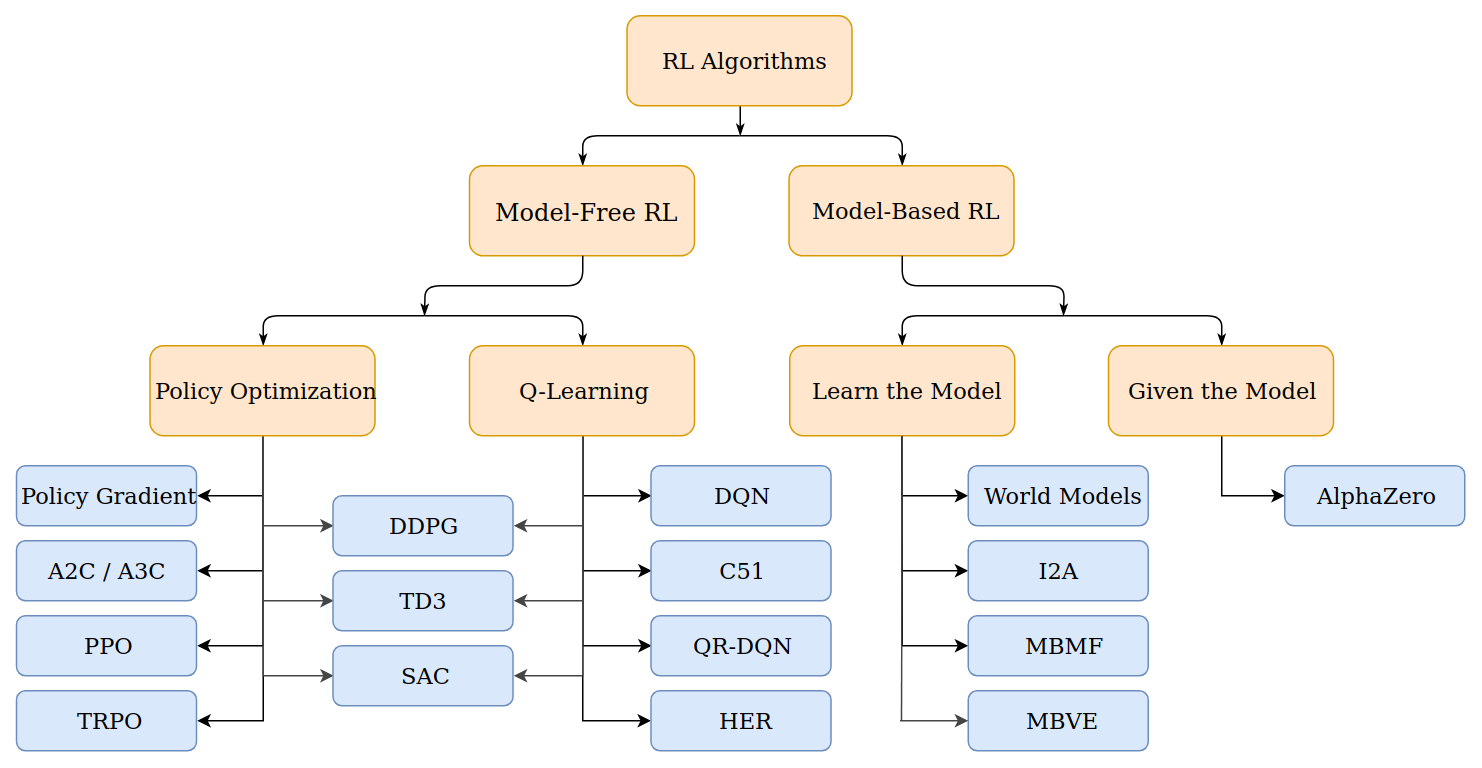
\includegraphics[height=6cm]{figures/taxonomy.png}
    \end{figure}
    \blfootnote{
        There are many partial taxonomies, this one is from~\cite{spinningup}.
    }
\end{frame}

\begin{frame}{A taxonomy of RL algorithms}
    \begin{figure}
        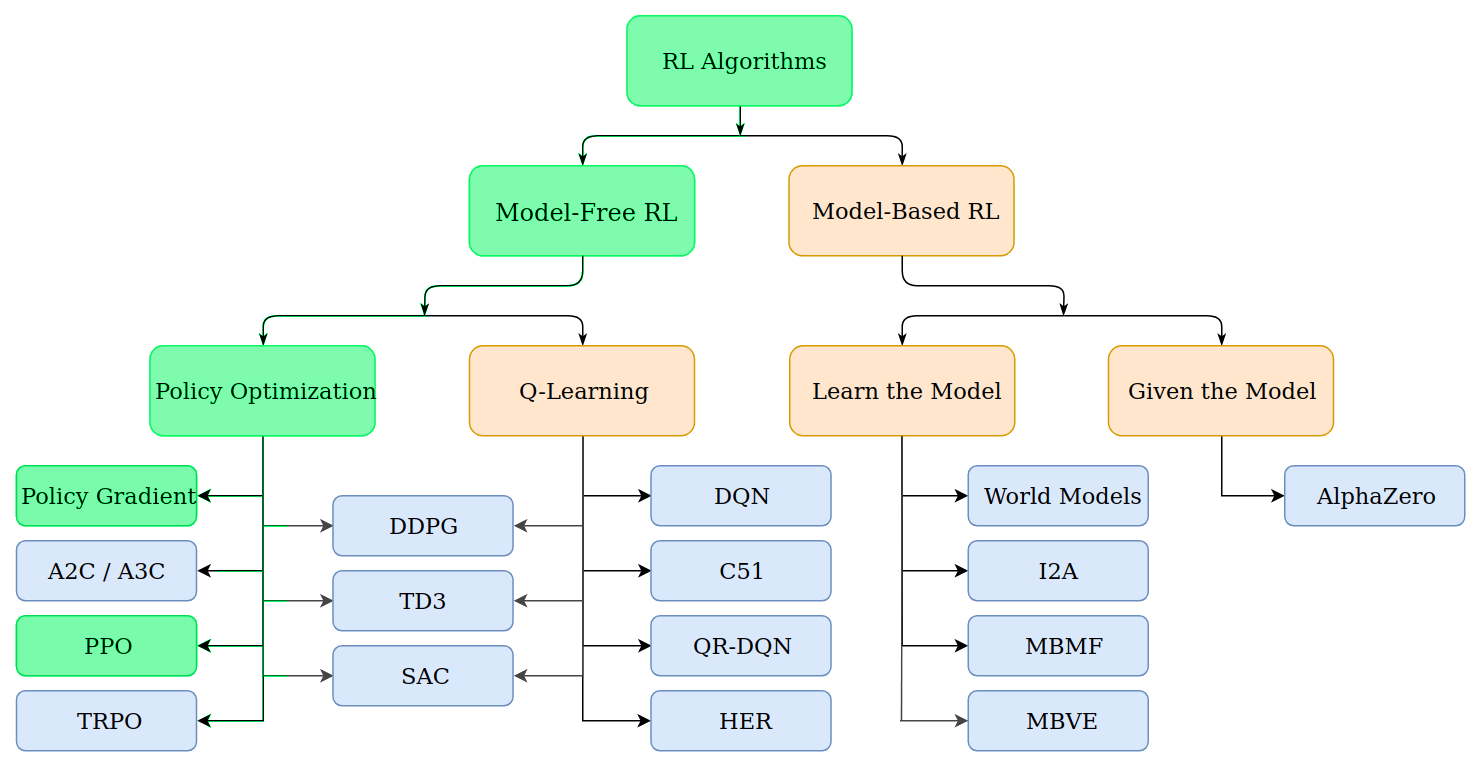
\includegraphics[height=6cm]{figures/taxonomy-focus.png}
    \end{figure}
    \blfootnote{
        Our focus in this class.
    }
\end{frame}

\section{Policy gradient algorithms}

\begin{frame}{Policy-based algorithms}
    Policy-based algorithms update a policy iteratively. At each iteration $k$:
    \begin{itemize}
        \item Collect trajectories $\mathcal{T}_k = \{ \tau \}$
        \item Update the policy $\pi_{k+1} = \mathit{update}(\pi_k, \mathcal{T}_k)$
    \end{itemize}
    Two ways to collect trajectories:
    \begin{itemize}
        \item \textbf{On-policy:} trajectories $\mathcal{T}_k$ are collected with the latest policy $\pi_k$
        \item \textbf{Off-policy:} trajectories $\mathcal{T}_k$ are collected with any policy
    \end{itemize}
\end{frame}

\begin{frame}{REINFORCE}
    \begin{block}{REINFORCE algorithm}
        \begin{itemize}
            \item \textbf{Input:} differentiable policy $\pi_\theta(a | s)$ parameterized by $\theta \in \mathbb{R}^n$
            \item \textbf{Parameter:} step size $\alpha > 0$
            \item Initialize policy parameters $\theta$ (e.g. to $0$)
            \item Loop forever (for each episode):
                \begin{itemize}
                    \item Roll out an episode $\tau = (s_0, a_0, \ldots, s_{N}, a_{N})$ following $\pi_\theta$
                    \item For each step $t \in \tau$:
                        \begin{itemize}
                            \item $R \leftarrow \sum_{t' = t + 1}^N \gamma^{t' - t - 1} r_{t'}$
                            \item $\theta \leftarrow \theta + \alpha \gamma^t R \nabla_\theta \log \pi_\theta(a_t | s_t)$
                        \end{itemize}
                \end{itemize}
        \end{itemize}
    \end{block}
    \blfootnote{
        See~\cite{sutton2018}, Chapter 13.
    }
\end{frame}

\begin{frame}{Why this update rule}
    \LARGE
    $$
    \theta \leftarrow \theta + \alpha \gamma^t R \nabla_\theta \log \pi_\theta(a_t | s_t) ?
    $$
\end{frame}

\begin{frame}{Remember the goal}
    The goal of RL is to find a \emph{policy} that \emph{maximizes} the expected return:
    $$
    J(\theta) = \max_\theta \mathbb{E}_{\tau \sim \pi_\theta}[R(\tau)]
    $$
    We do so by gradient ascent:
    $$
    \theta_{k+1} = \theta_k + \alpha \nabla_\theta J(\theta_k)
    $$
    The gradient $\nabla_\theta J$ with respect to policy parameters $\theta$ is called the \emph{policy gradient}.
\end{frame}

\begin{frame}{Remember the goal}
    \begin{block}{Theorem}
        The policy gradient can be computed from rewards $R(\tau)$ and the log-policy gradient $\nabla_\theta \log \pi_\theta$ as:
        \begin{equation*}
            \nabla_\theta J(\theta) = \mathbb{E}_{\tau \sim \pi_\theta} \left( 
            R(\tau)
            \sum_{s_t, a_t \in \tau} \nabla_\theta \log \pi_\theta(a_t | s_t)
            \right)
        \end{equation*}
    \end{block}
    LHS: the graal. RHS: things we observe ($R(\tau)$) or know by design ($\nabla_\theta \log \pi_\theta$).

    \textbf{Proof:} blackboard.
\end{frame}

\begin{frame}{Back to REINFORCE}
    Gradient ascent:
    $$
    \theta_{k+1} = \theta_k + \alpha \nabla_\theta J(\theta_k)
    $$
    From the policy gradient theorem, this is equivalent to:
    $$
    \theta_{k+1} = \theta_k + \alpha \mathbb{E}_{\tau \sim \pi_\theta} \left( 
            R(\tau)
            \sum_{s_t, a_t \in \tau} \nabla_\theta \log \pi_\theta(a_t | s_t)
            \right)
    $$
    REINFORCE drops the expectation:
    $$
    \theta_{k+1} = \theta_k + \alpha R(\tau_k) \sum_{s_t, a_t \in \tau_k} \nabla_\theta \log \pi_\theta(a_t | s_t)
    $$
\end{frame}

\begin{frame}
    \begin{block}{Vanilla policy gradient~\cite{spinningup}}
        \centering
        \scalebox{0.8}{
            \begin{algorithm}[H]
                \KwData{initial policy parameters $\theta_0$, initial value function parameters $\phi_0$}
                \For{$k = 0, 1, 2, \ldots$}{
                    Collect trajectories $\mathcal{D}_k = \{ \tau_i \}$ by running $\pi_\theta = \pi(\theta_k)$\;
                    Compute rewards-to-go $\hat{R}_t$ and advantage estimates $\hat{A}_t$ based on $V_{\phi_k}$\;
                    Estimate the policy gradient as $$\hat{g}_k = \frac{1}{|\mathcal{D}_k|} \sum_{\tau \in \mathcal{D}_k} \sum_{t=0}^T \nabla_\theta \log \left.\pi_\theta(a_t | s_t)\right|_{\theta_k} \hat{A}_t$$
                    \hspace{-0.75em} Update policy parameters by \emph{e.g.} gradient ascent, $\theta_{k+1} = \theta_k + \alpha_k \hat{g}_k$\;
                    Fit value function by regression on mean-square error: $$\phi_{k+1} = \arg \min_\phi \frac{1}{T |\mathcal{D}_k|} \sum_{\tau \in \mathcal{D}_k} \sum_{t=0}^T \left(V_\phi(s_t) - \hat{R}_t\right)^2$$
                }
            \end{algorithm}
        }
    \end{block}
    \vspace{-1.5em}
\end{frame}

\begin{frame}{Proximal policy optimization}
    \begin{figure}
        \includegraphics[height=6.5cm]{genfig/ppo.pdf}
    \end{figure}
    \vspace{-0.5cm}
    \blfootnote{
        Source: \url{https://spinningup.openai.com/en/latest/algorithms/ppo.html}
    }
\end{frame}

\begin{frame}{Let's practice!}
    \begin{figure}
        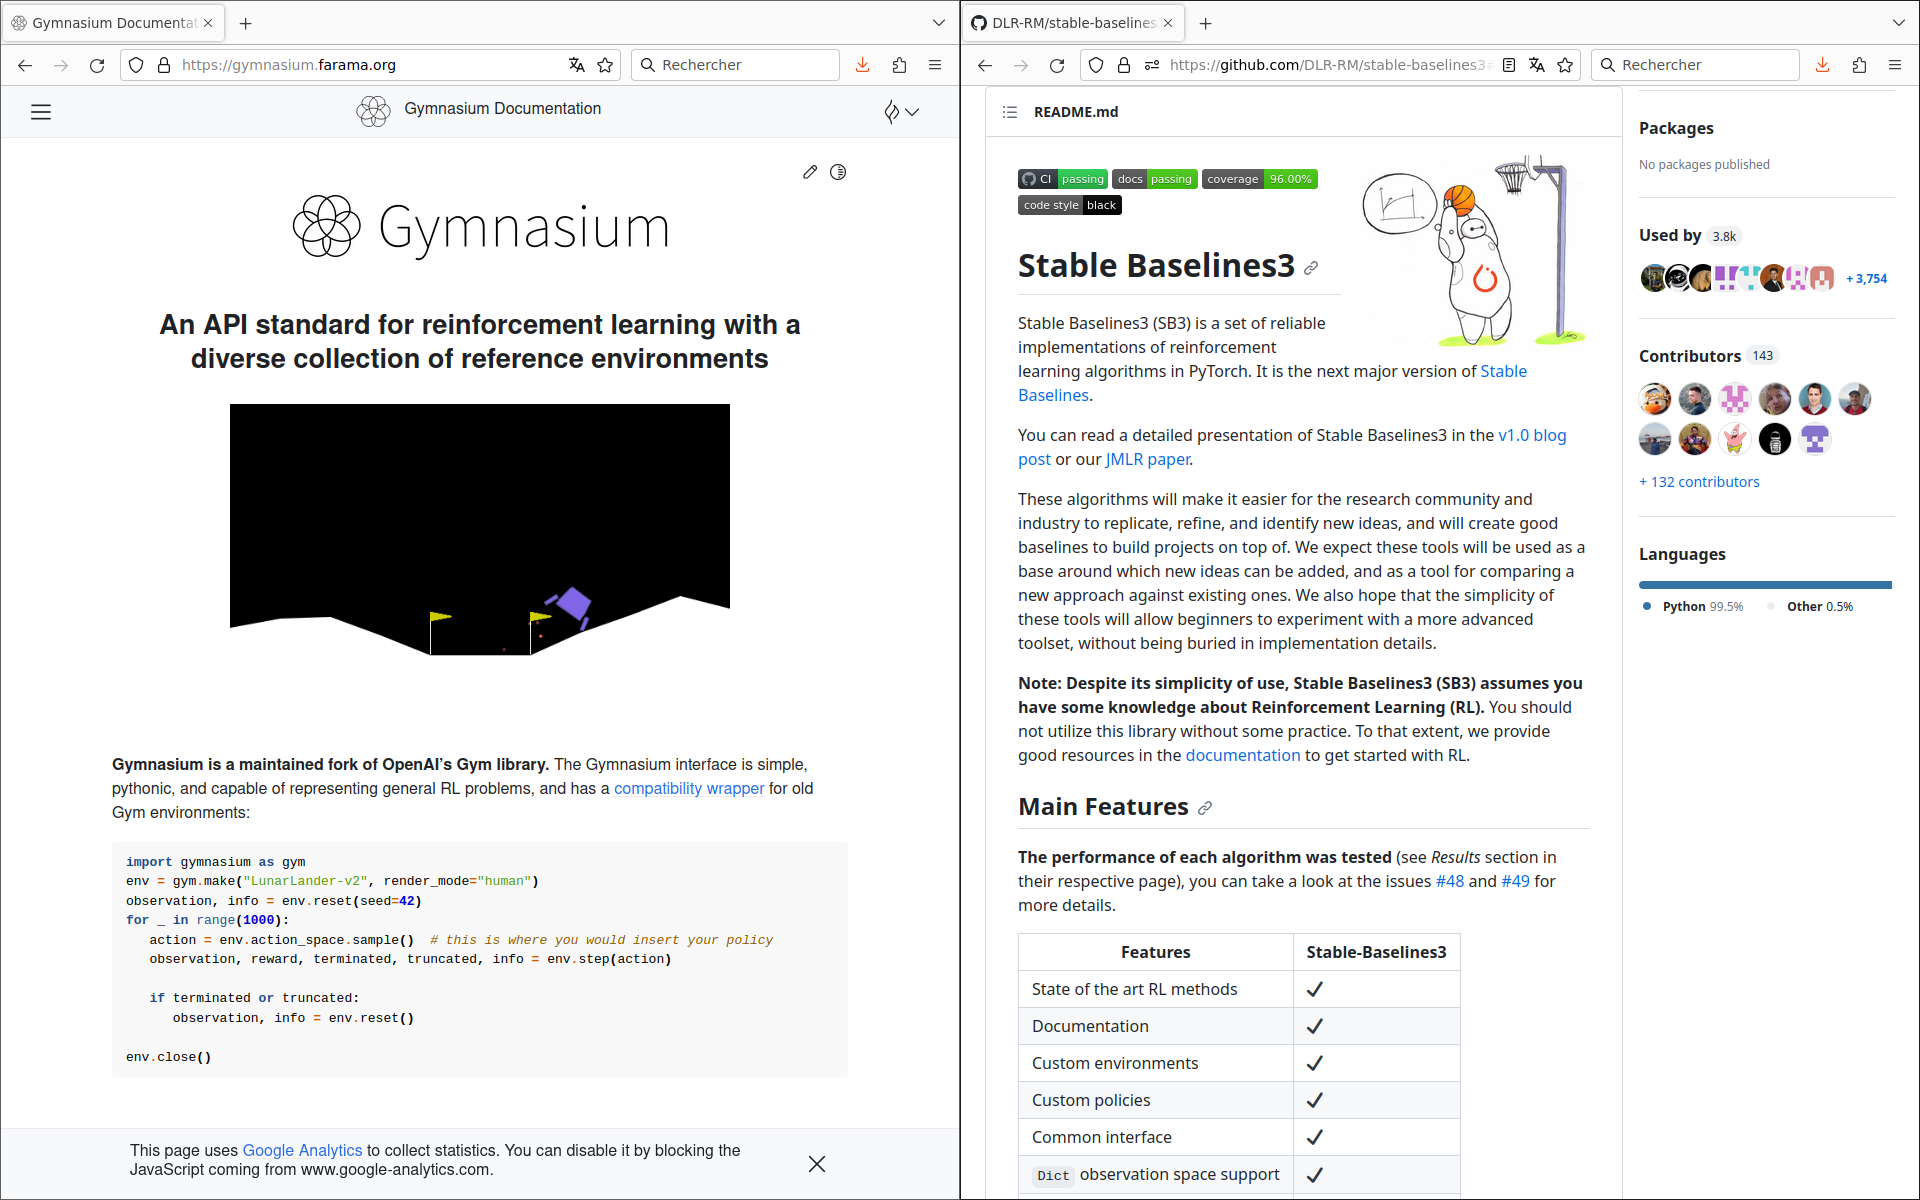
\includegraphics[width=0.99\columnwidth]{figures/gymnasium-sb3.png}
    \end{figure}
\end{frame}

\section{Application to robotics}

\begin{frame}{Quadrupedal locomotion~\cite{lee2020}}
    \begin{itemize}
        \item Residual reinforcement learning
        \item Hybrid physics/data-based simulation
        \item Domain randomization
        \item Observation and action noise
        \item Reward shaping
    \end{itemize}
\end{frame}

\begin{frame}{Quadrupedal locomotion~\cite{lee2020}}
    \vspace{1.5em}
    \begin{figure}
        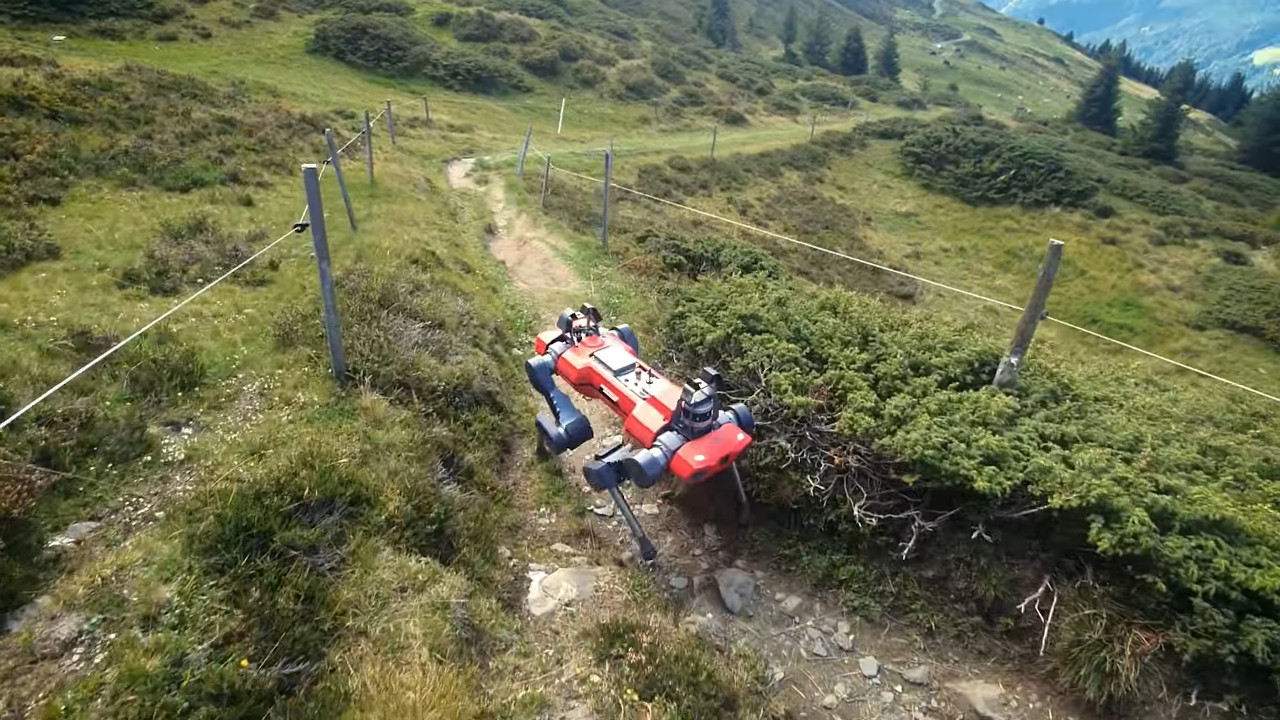
\includegraphics[height=5.5cm]{figures/hike-with-anymal.jpg}
    \end{figure}
    \begin{center}
        Teacher-student, residual reinforcement learning
    \end{center}
    \blfootnote{
        Video: \url{https://youtu.be/oPNkeoGMvAE}
    }
\end{frame}

\begin{frame}{Simulation pipeline}
    \begin{figure}
        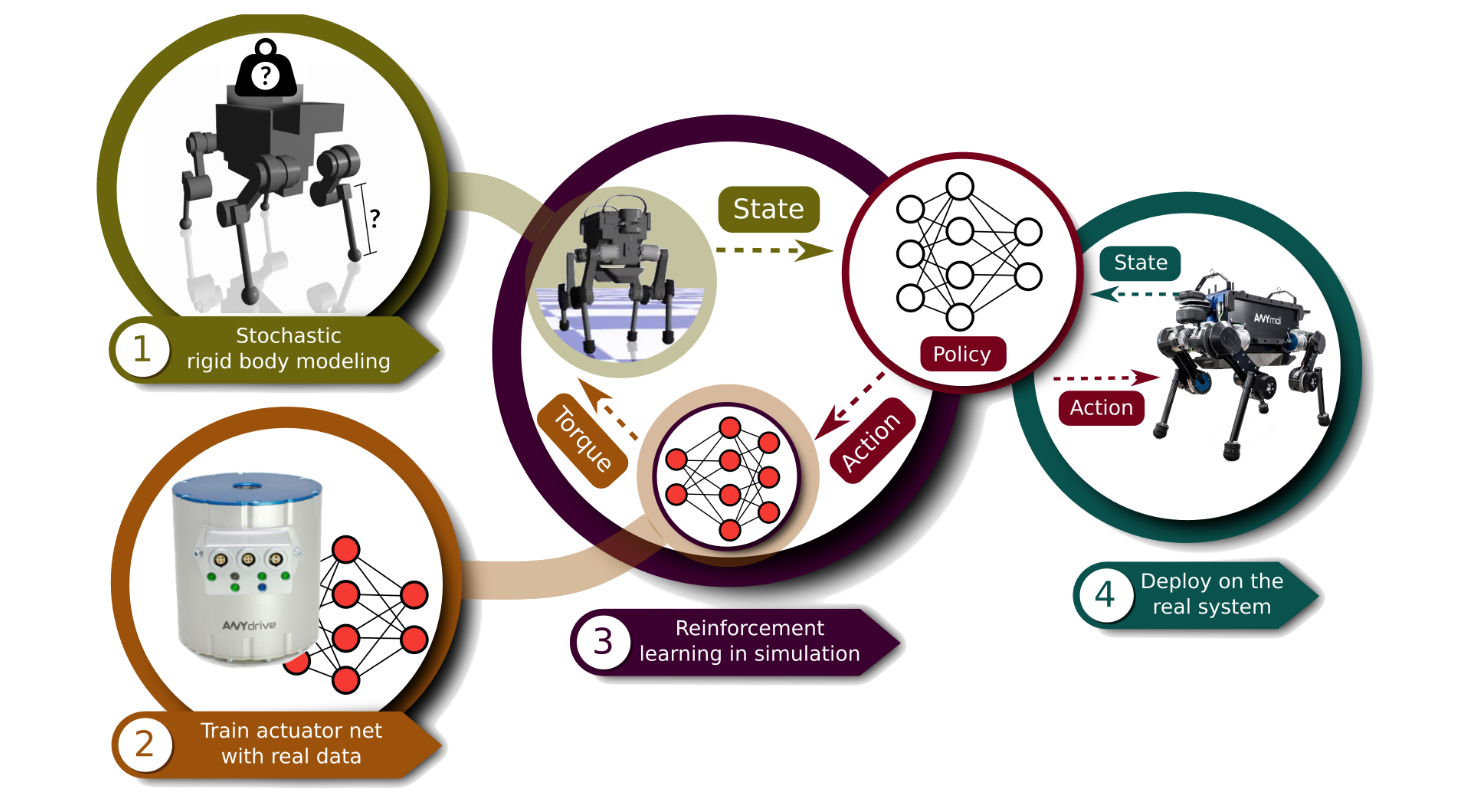
\includegraphics[height=6cm]{figures/quadruped-sim-pipeline.png}
    \end{figure}
    \blfootnote{
        Source:~\cite{hwangbo2019}
    }
\end{frame}

\begin{frame}{Training pipeline}
    \begin{figure}
        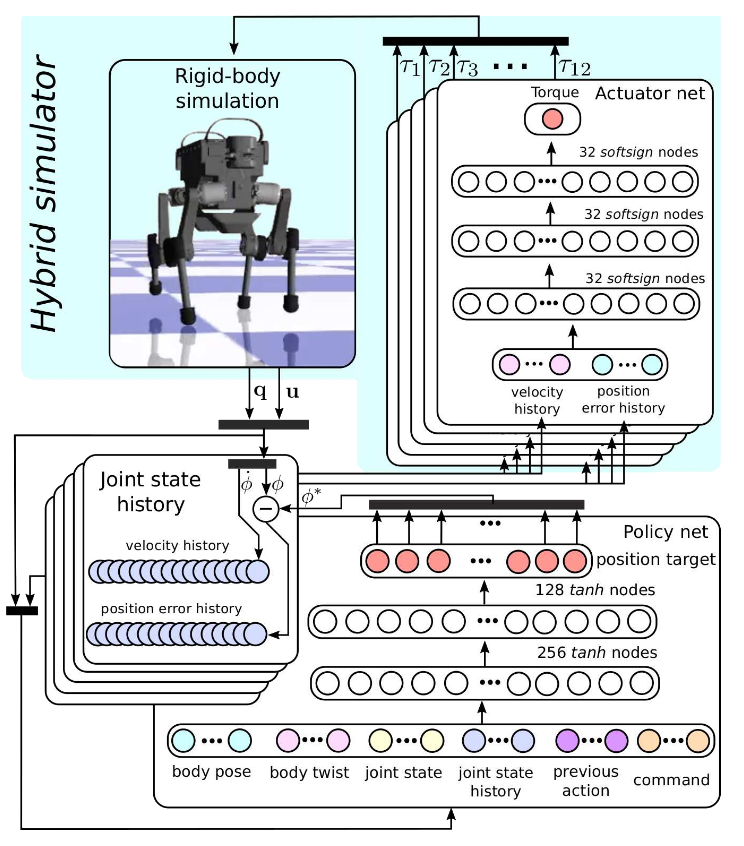
\includegraphics[height=6.7cm]{figures/quadruped-training.png}
    \end{figure}
    \vspace{-0.7cm}
    \blfootnote{
        Source:~\cite{hwangbo2019}
    }
\end{frame}

\begin{frame}{Curriculum}
    \begin{figure}
        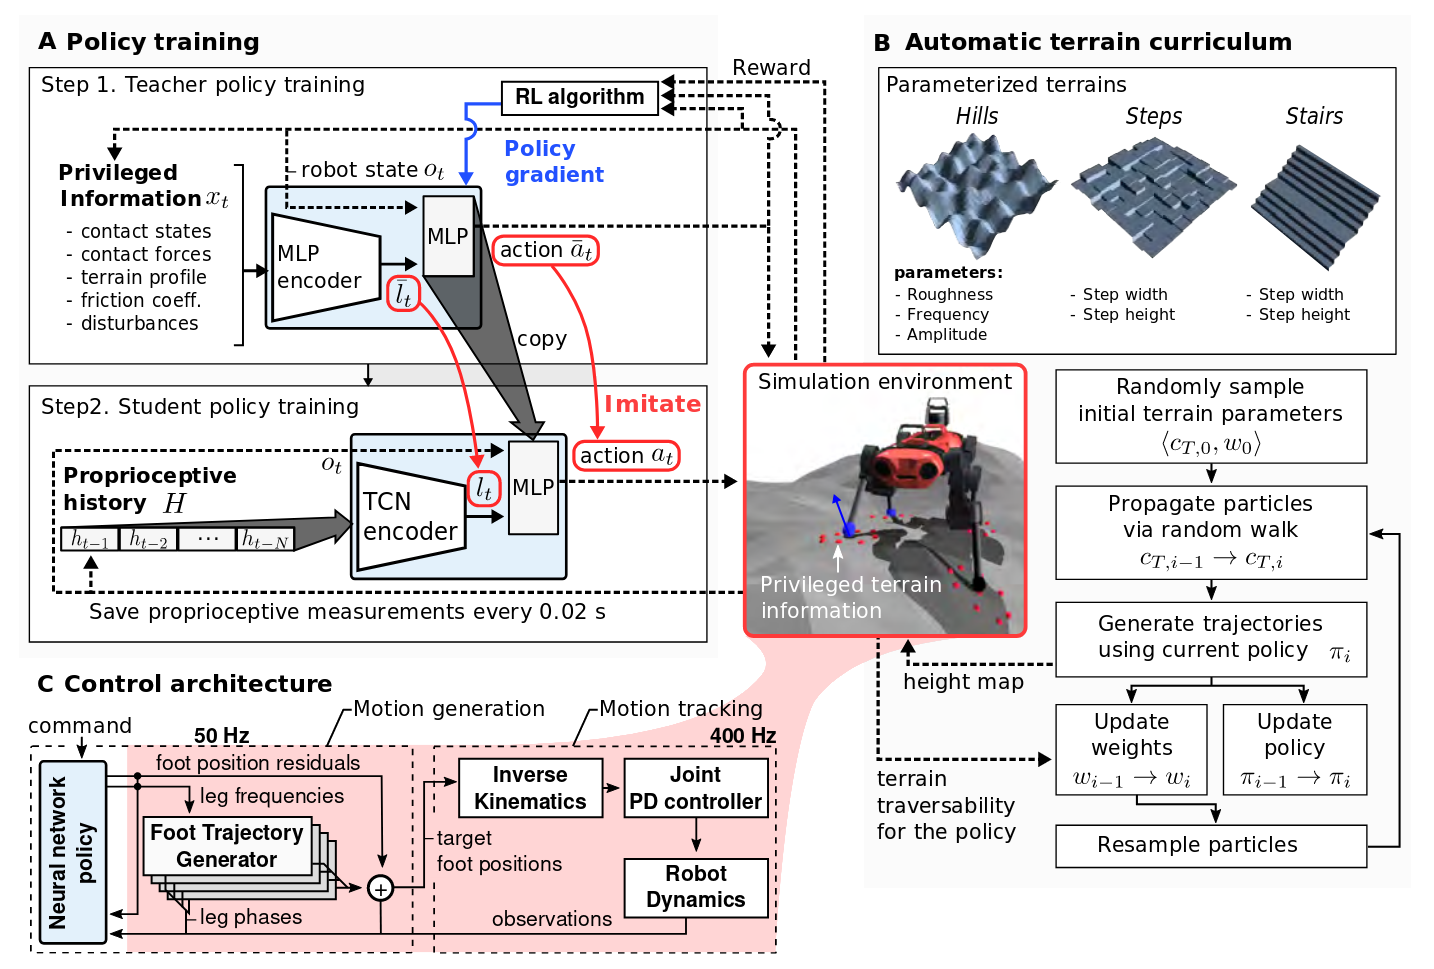
\includegraphics[height=6.7cm]{figures/quadruped-curriculum.png}
    \end{figure}
    \vspace{-0.7cm}
    \blfootnote{
        Source:~\cite{lee2020}
    }
\end{frame}

\begin{frame}{Formulating a reward}
    Let $r_e$ denote the reward associated with an error function $e$:

    Motivation:
    \begin{itemize}
        \item Exponential: $r_e = \exp(-e^2)$
    \end{itemize}

    Penalization:
    \begin{itemize}
        \item Absolute value $r_e = -|e|$
        \item Squared value: $r_e = -e^2$
    \end{itemize}
\end{frame}

\begin{frame}{RewArt}
    Making an RL pipeline work can lead to complex rewards, e.g. in~\cite{lee2020}:
    \begin{itemize}
        \item Linear velocity tracking: $r_{lv} = \exp(-2.0 (v_{pr} - 0.6)^2)$, or 1, or 0
        \item Angular velocity tracking: $r_{av} = \exp(-1.5 (\omega_{pr} - 0.6)^2)$, or 1
        \item Base motion tracking: $r_b = \exp(-1.5v_o^2) + \exp(-1.5 \|({}^B_{IB} \omega)_{xy}\|^2)$
        \item Foot clearance: $r_{fc} = \sum_{i \in I_{swing}} \mathbf{1}_{fclear}(i) / |I_{swing}|$
        \item Body-terrain collisions: $r_{bc} = -|I_{c,body} \textbackslash I_{c,foot}|$
        \item Foot acceleration smoothness: $r_{s} = -\| (r_{f,d})_t - 2(r_{f,d})_{t-1} + (r_{f,d})_{t-2}\|$
        \item Torque penalty: $r_{\tau} = -\sum_{i} | \tau_i |$
    \end{itemize}
    Final reward: $r = 0.05 r_{lv} + 0.05 r_{av} + 0.04 r_b + 0.01 r_{fc} + 0.02 r_{bc} + 0.025 r_s + 2 \cdot 10^{-5} r_{\tau}$
\end{frame}

\begin{frame}{Domain randomization}
    Randomize selected environment parameters
    \begin{itemize}
        \item Physical properties: geometry, inertias
        \item Initial state
    \end{itemize}
\end{frame}

\begin{frame}{Environment bounds}
    \begin{figure}
        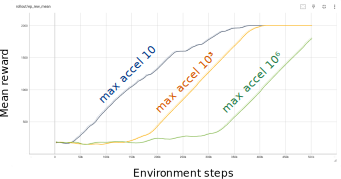
\includegraphics[width=0.99\columnwidth]{genfig/max-accel.pdf}
    \end{figure}
\end{frame}

\begin{frame}{Caveat: stochastic}
    \begin{figure}
        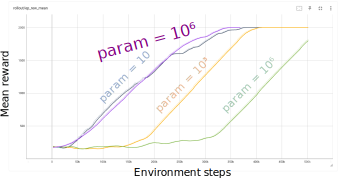
\includegraphics[width=0.99\columnwidth]{genfig/max-accel-bis.pdf}
    \end{figure}
\end{frame}

% \begin{frame}{Normalizing observations}
%     \begin{itemize}
%         \item Normalizing:
%         \item Standardizing:
%     \end{itemize}
% \end{frame}

\begin{frame}{Challenges for RL}
    \begin{itemize}
        \item \textbf{Sim2real:} no one-size-fits-all method, depends on robot and task
        \item \textbf{Jittering:} action noise, due to need for stochastic policies (PGT!)
        \item \textbf{Sample efficiency:} requires millions of samples $(s_t, a_t, s_{t+1})$
        \item \textbf{Reward shaping:} often a necessity, ``RewArt''!
        \item \textbf{Human supervision:} monitoring convergence to a satisfying policy\footnote{ Also known as SGD: ``Student Grad Descent``}
    \end{itemize}
\end{frame}

\section{Conclusion}

\begin{frame}{What we saw}
    \begin{itemize}
        \item Partially-observable Markov decision process (POMPD)
        \item The goal of reinforcement learning
        \item Model, policy and value function
        \item Policy gradient algorithm
        \item Application to robotics: residual RL, randomization, noise, rewart
        \item RL is not magic: great results, possibly going to great lengths!
    \end{itemize}
\end{frame}

\section*{Bibliography}

\renewcommand*{\bibfont}{\footnotesize}
\setbeamertemplate{bibliography item}{\insertbiblabel}
\begin{frame}[allowframebreaks]{References}
    \printbibliography[heading=none]
\end{frame}

\section*{Bonus: a rewarding triangle}

\begin{frame}[fragile]{A rewarding triangle}
    \begin{columns}
        \begin{column}{0.50\columnwidth}
            Environment:
            \begin{itemize}
                \item States: discrete triangle $\{(i, j), 0 \leq i < N, i \leq j \}$
                \item Rewards: $r_{i, j} \in \mathbb{N}$
                \item Initial state: $(0, 0)$
                \item Actions: $(i, j) \to (i + 1, j)$ or $(i, j) \to (i + 1, j + 1)$
            \end{itemize}
            What is the best return we can collect?
        \end{column}
        \begin{column}{0.50\columnwidth}
            Input: (first integer: $N$, then $N$ lines)
            \begin{minted}{bash}
                3
                1
                2 3
                4 5 6
            \end{minted}
            Output:
            \begin{minted}{bash}
                best_return=10
            \end{minted}
        \end{column}
    \end{columns}
    \blfootnote{
        Inputs: \url{https://scaron.info/robotique-mareva/triangles.zip}
    }
\end{frame}

\begin{frame}[fragile]{Your turn...}
    \begin{minted}{python}
        import numpy as np

        def value(triangle: np.ndarray, state: tuple) -> int:
            pass  # your job

        size = int(input())
        triangle = np.zeros((size, size), dtype=int)
        for row in range(size):
            rewards = [int(s) for s in input().split(" ")]
            for col, reward in enumerate(rewards):
                triangle[row, col] = reward

        best_return = value(triangle, state=(0, 0))
        print(f"{best_return=}")
    \end{minted}
\end{frame}

\begin{frame}{Example summary}
    \begin{itemize}
        \item \textbf{States:} triangle
        \item \textbf{Actions:} down or down-right
        \item \textbf{Observations:} full state
        \item \textbf{Model:} yes
        \item \textbf{Initial state:} $(0, 0)$
        \item \textbf{Value function:} yes
        \item \textbf{Policy:} greedy from value function
        \item \textbf{Return:} maximized
    \end{itemize}
\end{frame}

\end{document}
